
\documentclass[a4paper, 12pt]{article}
\usepackage{bm, array, graphicx, hyperref, amsmath, setspace, geometry, wrapfig}
\usepackage[font={footnotesize}]{caption}

\geometry{
a4paper,
total={170mm, 257mm},
left = 20mm,
top = 20mm
}

\begin{document}

\title{Cross relaxation mechanisms in fluorine-containing sample under conditions of DNP.}
\author{Dr Alexey Potapov\\
School of Physics and Astronomy\\
Sir Peter Mansfield Imaging Centre \\
\texttt{ alexey.potapov@nottingham.ac.uk}\\
tel: 0115 951 4739 }
\maketitle
 
\doublespacing
 
\section{Cross-relaxation in \textsuperscript{1}H- \textsuperscript{19}F system.}
While searching for optimal DNP conditions for DNP in fluorinated samples, we stumbled upon a peculiar phenomenon, where after shutting down the MW irradiation, the \textsuperscript{19}F magnetization builds up quickly to some higher than equilibrium value, then slowly reaches thermal equilibrium. These observations suggest that \textsuperscript{19}F nuclei are in contact with some other reservoir of energy, which is colder than lattice. The most obvious candidate for such a reservoir are abundant protons. This fact however, is yet to be fully confirmed.  
In the following we'll try to take a closer look at the mechanisms, which might be responsible for this transfer process.
\section{NOE.}
The transfer process is very similar to NOE (nuclear Overhauser effect), which has observed in solids quite a while ago. The latest reports published by the groups of Corzillius and Buntkowsky, describe NOE-like transfer from protons to carbons under conditions of MAS DNP (magnetic field of 9.4 T and temperature 100 K). Such transfer is induced by the motion of methyl groups, similarly other reports from the early days of NMR (Pines \& Waugh etc.) also attribute the transfer to some molecular motion. Our experiments however were carried at much lower temperatures of 1.4 K amplitudes, where motions are quite suppressed. 
Our main hypothesis is that \textsuperscript{1}H to \textsuperscript{19}F transfer is caused by the presence of paramagnetic TEMPO radical. When we inadvertently used  TEMPOL instead, we discovered that the \textsuperscript{1}H to \textsuperscript{19}F transfer was either significantly suppressed, or disappeared altogether. In order to show that in more detail we need to demonstrate what happens to the cross-polarization effect, when TEMPO concentration varies.

\section{Relaxation and Cross-relaxation.}
In the following we estimate the rates of cross-relaxation based on the time-dependent perturbation theory (Ch. VIII.II.C on Abragam's book). Consider a two a levelsystem, with $\vert i \rangle$ - initial, and $\vert f \rangle$ - final states, and the time-dependent perturbation to a system Hamiltonian $V(t) = \hat{A} f(t)$, where $\overline{f(t)} = 0$. The transfer rate from the $\vert i \rangle$ - to  $\vert f \rangle$ state can be calculated as:
\begin{equation} \label{eq:rate}
 W_{if} = \dfrac{ \vert A_{if} \vert ^2  }{\hbar^2} J(\omega_{if}) 
\end{equation}
where $\vert A_{if} \vert$ is the matrix element between the two states, and $J({\omega_{if}})$ is the spectral density at the transition frequency $\omega_{if} = \dfrac{E_f - E_i}{\hbar}$. For a stationary random process with exponentially decaying correlation function, the spectral density has the following form:
\begin{equation}
J(\omega) = \dfrac{\tau_c}{1+\omega^2\tau_c^2}, 
\end{equation} 
where $\tau_c$ is the correlation time of the random process.

In a three spin system, consisting of an electron and two nuclei, the pairwise interactions between all of them should be taken into account. However, in order to simplify the calculation we split this into two separate cases. 
\section{One hyperfine and one dipolar coupling} \label{sec: case A}
In this section we will consider a cross-relaxation mechanism arising due to rapid changes of nuclear spin quantization axis due to random electron spin flips. Random tilting of quantization axis affects the dipolar interaction between nuclear spins, giving rise to rapidly changing flip-flop terms.
In our calculation, we electron is coupled to a nearby proton via a hyperfine interaction, represented by a 2nd rank tensor $A_{ij}$ ($i,j=x,y,z$); the proton in turn is coupled to a nearby fluorine via a dipolar interaction with components $D_{ij}$ as shown schematically in Figure \ref{fig:coupling}A.

%%%% FIGURE COUPLING
\begin{figure}[b]
\caption{Interactions used to calculation. (A) Electron spin is hyperfine coupled to a proton, which is dipolar coupled to nearby fluorine. (B) Electron spin is hyperfine coupled to both a proton and a fluorine nuclei.}
\label{fig:coupling}
\centering
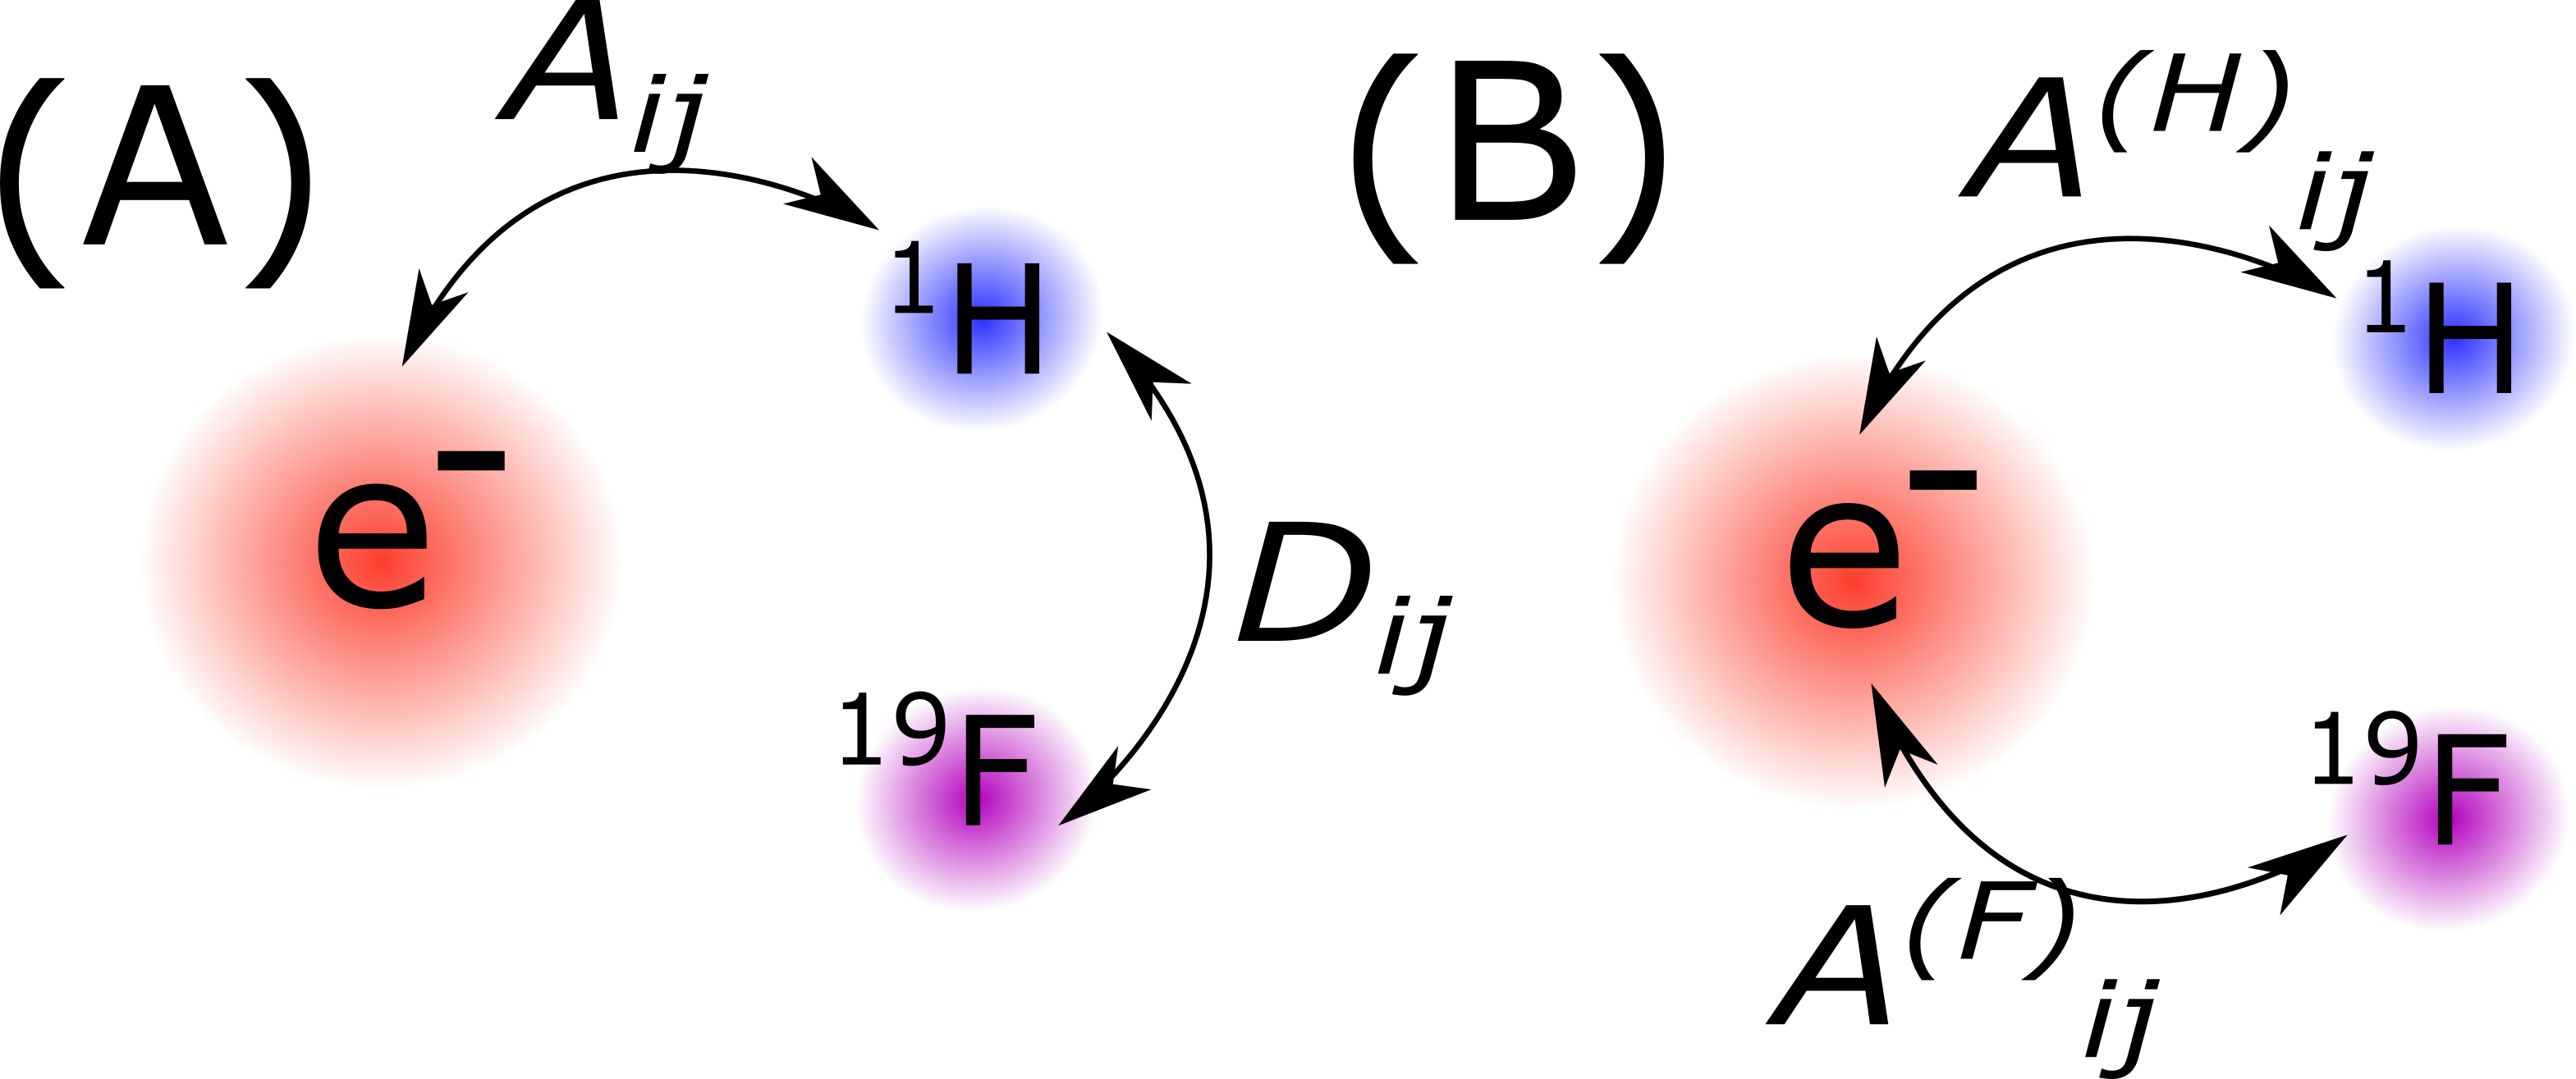
\includegraphics[scale=0.7]{text9330-7-6-8.png}
\end{figure}
%%%% END OF FIGURE

 We neglect the hyperfine interactions of \textsuperscript{19}F nuclei at this stage to simplify the calculation and evaluate the effect of hyperfine and dipolar interaction on relaxation exclusively. The spin Hamiltonian for such coupled three spin system can be written as: 
\begin{equation}
\mathcal{H} =  \omega_S \hat{S}_z + \sum_{i,j=x,y,z} A_{i,j} \hat{S}_i \hat{H}_j + \omega_H \hat{H}_z + \omega_F \hat{F}_z + \sum_{i,j=x,y,z} D_{ij} \hat{H}_i \hat{F}_j,
\end{equation}
where $\hat{H}_i, \hat{F}_i, \hat{S}_i$ - are the angular momenta of proton, fluorine and electron spins respectively. Taking into account that electron Zeeman interaction is greater than any other terms, the Hamiltonian in the electron spin rotating frame would take a form:
\begin{equation}
  \mathcal{H}  = A \hat{S}_z \hat{H}_z + B \hat{S}_z \hat{H}_x + D_{i,j} \hat{H}_i \hat{F}_j +  \omega_H \hat{H}_z + \omega \hat{F}_z + \sum D_{i,j} \hat{H}_i \hat{F}_j,
\end{equation}
where $A$ and $B$ are the secular and non-secular terms of the hyperfine interaction (term proportional to $\hat{S}_z \hat{H}_y$ was eliminated by a rotation in the spin space). The time-dependence in this Hamiltonian arises due to random flips of an electron spin, having a projection $m_S(t)=\pm \frac{1}{2}$ projection on the z-axis:
\begin{equation}
\mathcal{H} = (\omega_H + A m_S(t)) H_z + B H_x m_S(t) + + \omega \hat{F}_z + \sum D_{i,j} \hat{H}_i \hat{F}_j
\end{equation}
The first two terms would collectively correspond to quantization of a nuclear spin along a new effective magnetic field $\tilde{\mathbf{B}}=\dfrac{1}{\gamma}(\omega_H + A m_S(t)), \gamma B, 0)$. By rotating the spin operator around $H_y$ by a small angle $\phi(t)= arctan(\dfrac{m_S(t)B}{\omega_H + m_S(t) A} )  \approx \dfrac{m_S B}{\omega_H}$ one can rewrite this part of Hamiltonian along the new axis: $B_z(t) \hat{H}_z + B_x(t) \hat{H}_x = \tilde{\omega}_H(t) \hat{\tilde{H_z}}$. The $\hat{H}_y$ operator generates a rotation in the spin space, the dipolar part of the Hamiltonian can will then be transformed as:
\begin{equation}
\begin{array}{cc}
 \hat{\tilde{H}}_{dip} (t) =  exp(-i \phi(t) \hat{H}_y) \sum\limits_{i,j=x,y,z} D_{i,j} \hat{H}_i \hat{F}_j exp(i \phi(t) \hat{H}_y)  \approx  \\
\approx \phi(t)[ \sum \limits_{i,j=x,y,z} D_{ij} \hat{H}_i \hat{F}_j, \hat{H}_y] = \dfrac{m_S(t) B}{\omega_H} [ \sum \limits_{i,j=x,y,z} D_{ij} \hat{H}_i \hat{F}_j, \hat{H}_y]
\end{array}
\end{equation}
This time dependent Hamiltonian contains terms such as $\hat{H}_{\pm} \hat{F}_{\mp}$ and $\hat{H}_{\pm} \hat{F}_{\pm}$ is capable of inducing zero quantum (flip-flop) or double-quantum (flop-flop) transitions respectively. We will skip obtaining the exact equation for the rate, but rather focus in evaluating it by the order of magnitude. Using equation \ref{eq:rate} we can estimate the zero-quantum transfer rate as:
\begin{equation}
\begin{array}{cc}
W_{ZQ}  \sim \vert \dfrac{B D}{\omega_H} \vert ^2 J(\omega_{ZQ}) \\
J(\omega) = \dfrac{\tau_c}{1+\omega^2\tau_c^2}
\end{array}
\end{equation}
where $B$ - is non-secular proton hyperfine interaction, $D$ - dipolar coupling, $ZQ$ stands for zero-quantum ($\omega_{ZQ} = \omega_H - \omega_F$), $\tau_c$ - electron correlation time, which is case is determined by electron spin-diffusion ($\tau_c$ should be smaller than 100 $\mu s$ based on my CPMG measurements outlined in 2012 JMR paper - \textbf{this requires more explanations}). At the same time, the electron-induced $W_n = \dfrac{1}{T_{1n}}$ relaxation of \textsuperscript{19}F nuclei can be estimated as (Ch. IX.II.A Abragam):
\begin{equation}
W_{n}  \sim \vert B \vert ^2 J(\omega_F) \\
\end{equation}
Since $\omega_F \tau_c \gg 1$ and $\omega_{ZQ} \tau_c \gg 1$ ,  the spectral densities are equal to $J(\omega_F) \approx \dfrac{1}{\omega_F^2 \tau_c}$ and $J(\omega_{ZQ}) \approx \dfrac{1}{\omega_{ZQ}^2 \tau_c}$ . We can then look that the ratio of two rates, assuming that $\omega_H \approx \omega_F$:
\begin{equation}
\dfrac{W_{ZQ}}{W_n} \sim \vert \dfrac{D}{\omega_H} \vert^2 (\dfrac{\omega_F}{\omega_{ZQ}})^2 \sim (\dfrac{D}{\omega_{ZQ}})^2
\end{equation}
Since a typical dipolar coupling is $D \sim 100 \text{ kHz}$ and $\omega_{ZQ} \sim 8 \text{ MHz}$, then $W_{ZQ} \ll W_n$ i.e. the $ZQ$ process is several orders of magnitude slower than nuclear relaxation rate $\dfrac{1}{T_1}$ due to presence of electrons. Similar argument is true for for a double-quantum process. 

\section{Electron-induced proton-fluorine flip-flops}
Now we will include the hyperfine interactions for both nuclei, while neglecting the dipolar interaction between them as shown schematically in Figure \ref{fig:coupling}B. The Hamiltonian for such a system would therefore be in the following form:
\begin{equation}
\mathcal{H} =  \omega_S \hat{S}_z + \sum_{i,j=x,y,z} A_{ij}^{(H)} \hat{S}_i \hat{H}_j +  \sum_{i,j=x,y,z} A_{ij}^{(F)} \hat{S}_i \hat{H}_j + \omega_H \hat{H}_z + \omega \hat{F}_z ,
\end{equation}
where $A_{ij}^{(H)}, A_{ij}^{(F)}$ are the hyperfine interaction tensors of protons and fluorines respectively. In the electron spin rotating frame, using $A_{H,F}$ and $B_{H,F}$ for secular and non-secular terms of a hyperfine interaction the Hamiltonian can be rewritten as:
\begin{equation}
\mathcal{H}  = A_H \hat{S}_z \hat{H}_z + B_H \hat{S}_z \hat{H}_x +  \omega_H \hat{H}_z + A_F \hat{S}_z \hat{F}_z + B_F \hat{S}_z \hat{F}_x + \omega_F \hat{F}_z
\end{equation}
Since $B_H, B_F \ll \omega_H, \omega_F $, the non-secular terms can be regarded as a perturbation to a secular Hamiltonian. For simplicity, let's consider the action of this perturbation of an eigestate $\vert \Psi^{(0)} = \rangle  \vert \alpha_H \beta_F \rangle$. In the first order of perturbation theory, this function will transform into:

\begin{equation}
\Psi^{(1)}  =  \vert \alpha_H \beta_F \rangle  + c_1  \vert \beta_H \alpha_F \rangle + c_2  \vert \beta_H \alpha_F \rangle,
\end{equation}
where $c_1, c_2 \sim \dfrac{B_{H,F}}{\omega_{H,F}}$. All the mixed states differ from one another only by a flip of one nucleus. The second order of perturbation theory will mix addition states:
\begin{equation}
\Psi^{(2)}  =  \vert \alpha_H \beta_F \rangle  + c_1  \vert \alpha_H \alpha_F \rangle + c_2  \vert \beta_H \beta_F \rangle + d_1 \vert \beta_H \alpha_F \rangle + d_2(...\text{all other functions}...),
\end{equation}
The coefficient $d_1, d_2 \sim  \dfrac{B^2}{\omega^2}$, where $B$ is a combination of hyperfine couplings of protons and fluorines, and $\omega$ - the energy difference between the levels. 

Also, then increasing orders of perturbation theory corrections to the energy would produce terms of the order:
\begin{equation}
E ~ \sim \omega (1 + \dfrac{B}{\omega} + (\dfrac{B}{\omega})^2 + ...)
\end{equation}
The zeroth order correponds to a Zeeman interaction, the first order should be zero in our case. The second order correction would produce affective three spin terms in the Hamiltonian proportional to $S_z H_{\pm}F_{\mp}, S_z H_{\pm}F_{\pm}$ and having a magnitude of $\dfrac{B^2}{\omega} \sim 1 \text{ MHz} \gg D$. Such terms are time dependent and are capable to producing nuclear zero-quantum and double-quantum transitions respectively.
Similarly to section \ref{sec: case A} we can estimate the ratio of zero-quantum relaxation rate and the nuclear relaxation rate. 
\begin{equation}
\dfrac{W_{ZQ}}{W_n} \sim \vert \dfrac{B}{\omega_H} \vert^2 (\dfrac{\omega_F}{\omega_{ZQ}})^2 \sim (\dfrac{B}{\omega_{ZQ}})^2
\end{equation}
Hyperfine couplings of protons can be estimated as $B \sim \dfrac{78}{r^3} \dfrac{\text{ MHz} }{ \AA^3}  $, which for a distance of 2 $\AA$ would produce  a hyperfine coupling of about 10 MHz. In addition, the protons of nitroxide methyl groups have large anisotropic hyperfine couplings of about 10 MHz (J. Phys. Chem. 1982, 86, 4011). Altogether it means that proton nuclei with coupling on the order of  10 MHz are always present in the vicinity of TEMPO. Therefore the rate of a ZQ transition, or a flip-flop and relaxation rate due to presence of electrons,  will have the same order of magnitude as the electron-induce nuclear relaxation time $\dfrac{1}{T_{1n}}$.

\section{Conclusions.}
In this sketchy calculations we have compared two potential mechanisms for proton to fluorine magnetization transfer induced by the electron spin flips. When electron is strongly hyperfine coupled to both fluorine and proton nuclei, its fluctuations induce nuclei flip-flop transitions.

 
%
%\section{Definitions.}
%Experiments based on creating double-quantum coherence are quite often used in solution and solid-state NMR. Below we will consider the main principles underlying such experiments.
%As we know a system of two $I= \frac{1}{2}$ spins would form a system of 4 levels, which energies and eigenfunction can be calculated using the spin Hamiltonian:
%\begin{equation}
%\begin{array}{lcl}
%\hat{H} = \hat{H}_{dip} + \hat{H}_{CSA} \\
%\hat{H}_{dip} = \frac{\gamma_1 \gamma_2 }{r^3} (3 \hat{I}_{1z} \hat{I}_{2z} -  \hat{\bf{I}}_1 \hat{\bf{I}}_2) \\
%\hat{H}_{CSA} = \sum_{i,j = x,y,z} (1 - \sigma_{1i,j}) B_i \hat{I}_{1j}  +  \sum_{i,j = x,y,z} (1- \sigma_{2i,j} ) B_i \hat{I}_{2j}
%\end{array}
%\end{equation}
%The levels in a 4-level system will be some linear combinations of functions, corresponding to $\vert \alpha_1 \alpha_2  \rangle$, $\vert \alpha_1 \beta_2  \rangle$, $\vert \beta_1 \alpha_2  \rangle$, $\vert \beta_1 \beta_2  \rangle$ . For simplicity we will characterize the level with the function contributing the most. The transitions between the levels would be corresponding then to a flip of zero, one or two spins, thus they are named as zero-quantum (ZQ), single-quantum (SQ) and double-quantum (DQ) transitions.
%
%The density matrix describing the quantum state of such a two spin system will be a 4x4 matrix, where diagonal terms would correspond to population of corresponding levels, and off-diagonal terms are called \emph{coherences}. They show in fact how \emph{coherent} with one another the two states are. 
%\begin{equation}
%\rho = \left( \begin{array}{cccc} 
%   pop & SQ & SQ & DQ \\
%   SQ & pop & ZQ & SQ \\
%   SQ & ZQ & pop & SQ \\
%   DQ & SQ & SQ & pop 
%   \end{array}  \right)
%\end{equation} 
%The order of the coherence is inherited after a transition connecting two coherent states, so the coherence between 
%$\vert \alpha_1 \alpha_2  \rangle \leftrightarrow  \vert \alpha_1 \beta_2 \rangle$ is called a single-quantum, $\vert \beta_1 \alpha_2  \rangle \leftrightarrow  \vert \alpha_1 \beta_2 \rangle$ - zero quantum, $\vert \alpha_1 \alpha_2  \rangle \leftrightarrow  \vert \beta_1 \beta_2 \rangle$ is double-quantum coherence.
%
%Very often in NMR the evolution of the spin system goes under so-called double-quantum Hamiltonian, which has the following form: 
%\begin{equation}
%\hat{H}_{DQ} = d (\hat{I}_{1+} \hat{I}_{2+} + \hat{I}_{1-} \hat{I}_{2-} )
%\end{equation}
%Hamiltonian in such form may arise  in solid state NMR under the action of some rotor-synchronised sequences. It is quite easy to see that only $\vert alpha_1 \alpha_2 \rangle$  and  $\vert beta_1 \beta_2 \rangle$ are connected by this Hamiltonian. In the basis of $\vert \alpha_1 \alpha_2 \rangle $ etc. functions, its matrix would have the following form:
%
%\begin{equation}
%\hat{H}_{DQ} = d\left(
%\begin{array}{cccc}
%0 & 0 & 0 & 1 \\
%0 & 0 & 0 & 0 \\
%0 & 0 & 0 & 0 \\
%1 & 0 & 0 & 0 \\
%\end{array}
%\right)
%\end{equation}
%The matrix has a form very similar to $\hat{I}_x$ operator:
%\begin{equation}
%\hat{I}_x = \frac{1}{2}\left(
%\begin{array}{cc}
%  0 & 1\\
%  1 & 0
%\end{array}
%\right)
%\end{equation}
%$\hat{H}_{DQ}$ connects only $\vert 1 \rangle = \vert \alpha_1 \alpha_2 \rangle$ and $\vert 4 \rangle = \vert \beta_1 \beta_2 \rangle$ states, and we could represent it as being proportional to $ \hat{I}_{x}^{(1,4)} $ operator acting on $\vert 1 \rangle$  and $\vert 4 \rangle$:
%\begin{equation}
% I_{x}^{(1,4)} = \frac{1}{2} \left(
%\begin{array}{cccc}
%0 & 0 & 0 & 1 \\
%0 & 0 & 0 & 0 \\
%0 & 0 & 0 & 0 \\
%1 & 0 & 0 & 0 \\
%\end{array}
% \right)
%\end{equation}
%
%The initial state of a system can be described by a density matrix $\rho_0 \sim \hat{I}_1z + \hat{I}_2z$. In the $\vert \alpha_1 \beta_1 \rangle...$ basis the density matrix would be have a matrix: 
%\begin{equation}
%\rho_0 \sim \frac{1}{2}(\hat{I}_{1z} + \hat{I}_{2z}) = \hat{I}_{z}^{(1,4)} = \frac{1}{2} \left(
% \begin{array}{cccc}
% 1 & 0 & 0 & 0 \\
% 0 & 0 & 0 & 0 \\
% 0 & 0 & 0 & 0 \\
% 0 & 0 & 0 & -1  
% \end{array}
%\right)
%\end{equation}
%
%\section{Evolution under DQ Hamiltonian.}
%
%The density matrix $\rho(t)$ at any moment of time $t$  can be calculated as:
%\begin{equation}
%\begin{split}
%\rho(t) &= \exp (-i\hat{H}_{DQ}t) \rho_0  \exp (i\hat{H}_{DQ}t) \sim \\
% &\sim \exp (-i \omega_{DQ} t \hat{I}_{x}^{(1,4)}) \hat{I}_{z}^{(1,4)}  \exp (i \omega_{DQ} t \hat{I}_{x}^{(1,4)}) = \\
% &= \hat{I}_{z}^{(1,4)} \cos{\omega_{DQ} t} +  \hat{I}_{y}^{(1,4)} \sin{\omega_{DQ} t}, \\
% & \text{where } \omega_{DQ} = d/\hbar
%\end{split}
%\end{equation}
%
%The operator $\hat{I}_{y}^{(1,4)} = \frac{i}{2}( \hat{I}_{1+} \hat{I}_{2+} - \hat{I}_{1-} \hat{I}_{2-}) $ corresponds to a double-quantum coherence. A double-quantum operator therefore produces oscillations between the DQ coherence and a spin operator $\hat{I}_z^{(1,4)} = \frac{1}{2}(\hat{I}_{1z}+\hat{I}_{2z})$. In order to create the largest double-quantum coherence, one has to wait for delay $t_{max} = \frac{\pi}{2 \omega_{DQ}}$.
%
%\section{Double-quantum experiments}
%
%In the double-quantum-single quantum correlation experiment in solid-state NMR, the DQ coherence is first created using some specially designed sequence, such as POST-C7, SPC5 etc., which is followed by an evolution period, which selects only the DQ-coherence. The evolution of DQ coherence in the indirect dimension, which under MAS only contains isotropic chemical shifts, can be calculated as:
%
%\begin{equation} 
% \begin{split}
%  \rho(t) &= \exp[-i \hat{H}_{CS}t] \rho_0 \exp[ i \hat{H}_{CS}t] = \\
%  &=  \exp[-i(\omega_1 \hat{I}_{1z}  + \omega_2 \hat{I}_{2z})t] \frac{i}{2}( \hat{I}_{1+} \hat{I}_{2+} - \hat{I}_{1-} \hat{I}_{2-}) \exp[ i(\omega_1 \hat{I}_{1z}  + \omega_2 \hat{I}_{2z})t] = \\
%  &=  \frac{i}{2}( \hat{I}_{1+} \hat{I}_{2+} e^{i(\omega_1 t + \omega_2 t )} - \hat{I}_{1-} \hat{I}_{2-} e^{-i(\omega_1 t + \omega_2 t )}) 
% \end{split}
%\end{equation}
%
%As follows from these equations, the DQ coherence acquires phases proportional to sums of chemical shift frequencies, $(\omega_1 + omega_2)$. After the evolution of DQ coherences, they are being reconverted with a Hamiltonian $-\hat{H}_DQ$ back to $\hat{I}_{1z} + \hat{I}_{2z}$, which is being detected. In rotor-synchronized SPC5, POST-C7 etc. sequences the sign of effective Hamiltonian can be changed by changing the phases of all the pulses by $90 ^\circ$:
%\begin{eqnarray}
%\exp [-i \frac{\pi}{2} (\hat{I}_{1z}+\hat{I}_{2z})] \hat{H}_{DQ} \exp [i \frac{\pi}{2} (\hat{I}_{1z}+\hat{I}_{2z})]= d (\hat{I}_{1+} \hat{I}_{2+} e^{\pi}+ \hat{I}_{1-} \hat{I}_{2-} e^{-\pi}) = -\hat{H}_{DQ}
%\end{eqnarray}
%
%Double-quantum coherence can omly be created  between pairs of coupled spins. Therefore, NMR signals from spins, not coupled to any neighbors, such as natural abundance  \textsuperscript{13}C, and \textsuperscript{15}C nuclei etc. can be very efficiently filtered out. 
%The DQ filtering sequence would then be composed of a DQ production part, followed immediately by a DQ reconversion part, assuming that such sequence is long enough and coherences from uncoupled spins decay very quickly. 

%\section{Introduction.}



%%%% FIGURE SLICHTER PRECESSION
%\begin{wrapfigure}{1}{0.25\textwidth}
%\includegraphics[width=0.9\linewidth]{Slichter.png}
%\end{wrapfigure}
%%%% END OF FIGURE

%Magnetic resonance is an effect of transitions between levels of nuclear (or electron) spins induced by a resonant irradiation. Magnetic resonance effect is  widely used for probing the structure and dynamics of various materials and molecules at a level of individual atoms. It has enormous number of applications in physics, chemistry, biology and medicine, and the associated techniques have quite long ago stepped out of a domain of exclusively academic interest and become adopted by various industries.

%Below we will look into main concepts of magnetic resonance interleaved with some discussion of its current applications and comments on the roles (or jobs) where physicists could apply their skills. These lecture notes are not a complete overview of the field, however, it hopefully provides a good starting point for further exploration to those who get interested.
%
%\textbf{Suggested reading:} C.P. Slichter, Principles of Magnetic Resonance (3rd ed.)
%
%\section{Larmor Precession. Spin in a Magnetic Field.}
%Magnetic moment arises in the system of charges moving in a limited volume. The position of a charge $\bm{e_n}$ will be given by a vector $\bm{r_n}$ and its velocity by $\bm{v_n}$. The overall magnetic moment of such a system is defined as (in CGS):
%
%\begin{equation}
%\bm{M} = \frac{1}{2c} \sum_{n} e_n\bm{r_n} \times \bm{v_n}
%\end{equation}
%
%If all the charges and masses are the same, then $\bm{M}$ can be rewritten as:
%\begin{equation} \label{eq:1}
%\bm{M} = \frac{e}{2mc} \sum_{n} m\bm{r_n} \times \bm{v_n} = \gamma \bm{J},
%\end{equation}
%where
%\begin{equation}
%\bm{J} = \sum_{n} \bm{p_n} \times \bm{r_n}
%\end{equation}
%is the mechanical angular momentum. The ratio between the magnetic and mechanical moments is called a gyromagnetic ratio $\gamma = \frac{e}{2mc}$ (in fact it is a magnetogyric ratio, but for historical reasons it is rarely called so).
%When the abovementioned system of moving charges is placed into an external uniform permanent magnetic field $\bm{H}$, its energy is given by:
%
%\begin{equation} \label{eq:2}
%E = -\bm{M} \cdot \bm{H}
%\end{equation}
%The direction of a magnetic moment in this case is not constant. The torque acting on the system, produces a change in the mechanical angular momentum:
%\begin{equation}
%\frac{d\bm{J}}{dt} = \bm{M} \times \bm{H}
%\end{equation}
%Now using equation \ref{eq:1} we can obtain the equation governing the motion of vector $\bm{M}$:
%
%\begin{equation} \label{eq:precession_compact}
%\frac{d\bm{M}}{dt} = \gamma \bm{M} \times \bm{H}
%\end{equation}
%For an important case of a uniform magnetic field directed along $z$-axis $\bm{H} = (0, 0, H_0)$, a change in the magnetic moment components becomes:

%\begin{equation} \label{precession}
%\begin{array}{lcl}
%\dfrac{dM_x}{dt} & = & \omega_0 M_y \\
%\dfrac{dM_y}{dt} & = & -\omega_0 M_x \\
%\dfrac{dM_z}{dt} & = & 0,
%\end{array}
%\end{equation}
%where $\gamma H_0$ is denoted as $\omega_0$ for compactness.
%A solution to this system of differential equations with initial values of $M_x(0), M_y(0), M_z(0)$ has the following form:
%
%\begin{equation} 
%\begin{array}{lcl}
%M_x(t) &=& M_x(0) \cos(\omega_0 t) + M_y(0) \sin (\omega_0 t) \\
%M_y(t) &=& -M_y(0) \sin(\omega_0 t) + M_y(0) \cos (\omega_0 t) \\
%M_z(t) &=& M_z(0) 
%\end{array}
%\end{equation}

%These equations describe a precession of a vector $\bm{M}$ around the direction of the external magnetic field $\bm{H}$ with the frequency $\omega_0$ as shown schematically in Fig.\ref{fig:precession}A. Such motion is called  "Larmor precession" and $\omega_0$ is called "Larmor frequency".
%
%Of course, this primitive classical picture serves only as an illustration to the actual behaviour of magnetic moments placed into a magnetic field. However, a more rigorous description using quantum mechanics for an ensemble of magnetic moments provides a similar answer. Larmor precession of an overall magnetic moment is a real effect, and as we will see later, it is essential for acquiring of magnetic resonance spectra.
%
%%%%% FIGURE LARMOR PRECESSION
%\begin{figure}[ht]
%\caption{(A) Magnetic moment precesses around the direction of a magnetic field with Larmor frequency. (B) The splitting between two levels of a spin-$\frac{1}{2}$ system grows linearly with the magnetic field.}
%\label{fig:precession}
%\centering
%%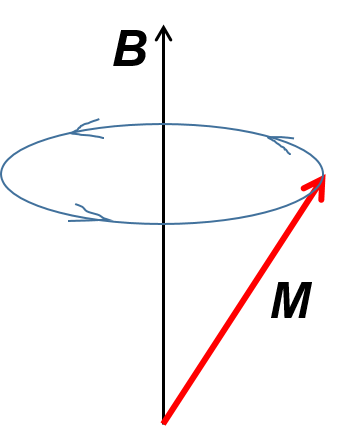
\includegraphics[scale=0.7]{precession.png}
%\end{figure}
%%%%% END OF FIGURE
%
%Without going deep into the quantum mechanics of precessing magnetic moments, we will remind ourselves of an angular momentum Hamiltonian in a magnetic field. The angular momentum operator $\bm{I}$ (which could be an orbital or spin angular momentum) is proportional to the magnetic moment operator as:
%\begin{equation} \label{eq:3}
%\bm{\hat{\mu}} = \gamma \hbar \bm{\hat{I}},
%\end{equation}
%The expression for energy in equation \ref{eq:2} can be replaced by a Hamiltonian:
%\begin{equation} \label{eq:2level}
%\hat{H} = -\bm{\hat{\mu}} \bm{H} = -\gamma \hbar \hat{I_z} H_0 = -\omega_0 \hat{I_z},
%\end{equation}
%
%The level diagram in Fig.\ref{fig:precession}B shows schematically the splitting of $\gamma \hbar H_0 $ between energy levels  as a function of the applied magnetic field for a system with  a spin-$\frac{1}{2}$ angular momentum only. In this case, the eigenfunctions corresponding to the two energy levels are just the two projections of a spin onto the $z$-axis: $m_z=+\frac{1}{2}$ is $\vert \alpha \rangle$ and $m_z=-\frac{1}{2}$ is $\vert \beta \rangle$.
%
%\textbf{Further reading:} Slichter, Ch. 2.1, 1.2 
%
%\section{Magnetic moments of nuclei.}
%Most nuclei have a spin angular momentum. In fact, nuclei consist of several spin-$\frac{1}{2}$ protons and neutrons, which sum up to give rise to an overall nuclear spin, which could have integer and half-integer values $I=0, \frac{1}{2}, 1, \frac{3}{2}, 2, \frac{5}{2}...$ A nucleus with a spin also has a magnetic moment, and similarly to \ref{eq:3} we can write:
%\begin{equation}
%\bm{\hat{\mu}_N} = -\gamma_N \hbar \bm{\hat{I}},
%\end{equation}
%where $\gamma_N$ is the nuclear gyromagnetic ratio, which is different for each nucleus, and $\bm{I}$ is the quantum mechanical spin angular momentum operator (rather than angular momentum related to some internal motion). Table \ref{tab:mag_properties} shows magnetic properties of several very common nuclei. Note that one of the columns shows their Larmor frequency at the magnetic field of 11.774 T. This field is very common for high-resolution nuclear magnetic resonance (NMR) experiments in liquids and solids. The Larmor frequencies belong to a radiofrequency range, which obviously dictates the use of an experimental apparatus suitable for sensitive detection at these frequencies. 
%
%% TABLE OF MAGNETIC PROPERTIES
%\begin{table}[ht]
%\caption{Magnetic properties of some common nuclei. More can be found at \url{http://www.bruker-nmr.de/guide/eNMR/chem/NMRnuclei.htm} }
%\label{tab:mag_properties}
%\centering
%\begin{tabular}{m{1.5cm} m{1.5cm} m{1.5cm} m{3cm} m{3cm}}
%\hline\hline
%Nucleus & Natural abundance \% & Nuclear spin (I) & Larmor frequency at 11.744T, MHz & Gyromagnetic ratio ($10^7$ rad/T*s) \\
%\hline
%\textsuperscript{1}H & 99.98 & $\frac{1}{2}$ & 500 & 26.7519 \\
%\textsuperscript{2}H & 1.5*10\textsuperscript{-2} & 1 & 76.753 & 4.1066 \\
%\textsuperscript{13}C & 1.108 & $\frac{1}{2}$ & 125.721 & 6.7283 \\
%\textsuperscript{14}N & 99.635 & 1 & 36.118 & 1.9338 \\
%\textsuperscript{15}N & 0.365 &  $\frac{1}{2}$ & 50.664 & -2.712 \\
%\textsuperscript{35}Cl & 75.53 &  $\frac{3}{2}$ & 48.991 & 2.624 \\
%\textsuperscript{37}Cl & 24.47 &  $\frac{3}{2}$ & 40.779 & 2.1842 \\
%\hline
%\end{tabular}
%\end{table}
%%%%%% END OF TABLE
%
%%%%%%RESONANT ABSORBTION SECTION
%\section{Resonant absorption.} \label{Res_absorbtion}
%
% In order to probe the energy levels of a nuclear spin system one could use electromagnetic irradiation. The magnetic component of an electromagnetic wave is the only relevant component in this case. A spin system Hamiltonian becomes time-dependent and for an oscillation along the $x$-axis we obtain:
%\begin{equation} \label{eq:oscillating_field}
%\begin{array}{lcl}
%\hat{H}(t) &=& -\bm{\hat{\mu}} \bm{(H_0+H(t))}=  \\
% &=& -\gamma \hbar \hat{I_z} (H_0 + H_1(t)) =\\
% &=&-\gamma \hbar \hat{I_z} H_0  -\gamma \hbar \hat{I_x} H_1 \cos(\omega t),
%\end{array}
%\end{equation}
%where $H_1$ and $\omega$ are the amplitude and the frequency of the oscillating magnetic field. According to perturbation theory the transition probability between the initial state $\vert a \rangle$ and the final state $\vert b \rangle$ with a time dependent Hamiltonian $ \kappa (t) = 2 \hat{F} \cos (\omega t ) $ is:
%\begin{equation} \label{eq:probability}
%P_{ab} = \frac{2 \pi}{\hbar} \vert \langle a \vert \hat{F} \vert \rangle b \vert ^2 \delta(E_{ab}-\hbar \omega),
%\end{equation}
%where $E_{ab} = E_a - E_b$ is an energy difference between the energies of levels $a$ and $b$. Obviously, the transition takes place only when the irradiation frequency $\omega$ exactly matches the difference in the energy of levels. For a spin $I = \frac{1}{2}$ system there are only two levels as shown in Fig.\ref{fig:precession} with corresponding eigenfunctions $\vert \beta \rangle$ and $\vert \beta \rangle$, which give a matrix element $\langle \alpha\vert \hat{I_x} \vert \beta \rangle = \frac{1}{2}$. The transition probability then becomes:
%\begin{equation}
%P_{ab} = \frac{\pi}{2\hbar} (\gamma H_1)^2 \delta(E_{ab}-\hbar \omega),
%\end{equation}
% \textbf{The effect of resonant absorption (and emission) of electromagnetic irradiation at the frequency matching the energy difference in a nuclear system is called Nuclear Magnetic Resonance (NMR).} The effect gives a name to the field of NMR spectroscopy, which is a general term for learning about nuclei in a sample through examining their energy spectra in the magnetic field. One could imagine an experimental apparatus where the frequency of electromagnetic irradiation  is scanned through a resonant region and absorption is detected. Such experiments were indeed carried out in the early days of NMR and are still now being used to detect spectra of unpaired electrons in a magnetic field (usually called Electron Paramagnetic Resonance or EPR). However, modern equipment uses somewhat other principles which will be discussed a little later.
%
%\textbf{Further reading:} Slichter, Ch. 1.3 
%%%%%% END OF RESONANT ABSORPTION
%
%\section{Chemical Shifts and $J$-couplings.}
% The strength of NMR signals can be used to tell how many spins are contained in a sample, which can very often be useful in quantitative analysis of various samples. But the power of NMR spectroscopy comes from the fact that almost every nucleus has a slightly different frequency depending on its environment. The spectral lines corresponding to these nuclei would be somewhat shifted away from their Larmor frequency. The shift is called \textbf{chemical shift} and is denoted as $\sigma$ in the Hamiltonian:
%
%\begin{equation}
%\hat{H} = -\gamma_N (1 - \sigma) H_0 \hat{I_z}
%\end{equation}
%
%Strictly speaking, chemical shifts in solids are 2nd-rank tensor, but in a simple case of liquids it only has one component, which is usually measured in parts per million (ppm). Chemical shift arises when molecular electron currents adjust to shield the external magnetic fields, thereby creating a somewhat different magnetic field at the nucleus location. The degree of shielding depends on the configuration of electrons, which is associated with molecular structure.
%
% There also other interactions, which revealing themselves in the spectra. A nuclear magnetic moment creates a magnetic field, which slightly disturbs electron orbitals, producing a slightly different local magnetic field at another nucleus. This electron-mediated mechanism creates a so called $J$ - coupling between two distant nuclei. Such interaction is usually added to a spin Hamiltonian as:
%
%\begin{equation}
%\hat{H}_J = J \bm{I_1} \bm{I_2},
%\end{equation}
%where $\bm{I_1}$, $\bm{I_2}$ are the spin angular momentum operators of the first and second nucleus, and $J$ is the coupling. As can be shown by solving a full spin Hamiltonian $J$-couplings produce noticeable splittings of spectral lines.
%
%  The discovery of chemical shifts and $J$-couplings was extremely important for chemistry and other related fields because chemical shifts together with $J$-couplings produce spectra, which could be used as unique fingerprints of molecules. Fig.\ref{fig:ethanol} shows a \textsuperscript{1}H NMR spectrum of an ethanol molecule, which has distinct chemical shifts for each of its protons, and groups of protons interacting with one another give rise to $J$-splittings in the spectra. 
%  
%%%%% FIGURE ETHANOL
%\begin{figure}[h]
%\caption{\textsuperscript{1}H-NMR spectrum of ethanol. Insert shows a structure of ethanol molecule. Horizontal axis are labelled in units of chemical shift (ppm) which is a usual way of presenting data in NMR}
%\label{fig:ethanol}
%\centering
%%\includegraphics[scale=0.7]{ethanol_Figure.png}
%\end{figure}
%%%%% END OF FIGURE
%
%  Spectra of larger molecules are much more complicated because of a larger number of contributing nuclei, however, there are approaches allowing to  resolve the spectra of large biomolecules and obtain their structures based on that information.
%  
%\textbf{Further reading:} Slichter, Ch. 4.4, 4.9 
%
%\section{Comment on the applications of NMR spectroscopy.}
%
%Much of fundamental physics related to magnetic resonance has been established in 1940-1960s, which led to lots of applications (predominantly in chemistry-related areas). There is still however quite many areas where physicists could apply their skills and expertise.
% 
%a. NMR spectroscopy can tell a lot about many biophysical processes taking place on the level of individual molecules. There is a very high interest in structures of large biomolecules, particularly proteins, because understanding of these structures can explain their functional properties. In turn, knowing those properties is important because of the clues they provide  for a more intelligent search of drugs affecting the function or dysfunction of its target and leading to treatment as a result.
%
%Structures of thousands of proteins have been revealed using NMR and now have been deposited into publicly available databases(such as PDB). Just one interesting example is a structure of so-called A$\beta$ amyloid fibrils, which were discovered in plaques forming the brains of Alzheimer's disease patients. Alzheimer's disease is a form of senile dementia and poses a serious heath threat to the world's ageing population, which is why so much effort of the research community is directed towards understanding the molecular origins of the disease. 
%
%Since 1980's people knew that fibrils associated with Alzheimer's disease are made of many copies of a protein called A$\beta$, however its exact arrangement within a fibril remained mysterious for a long time. Only recently, in the early 2000's, full atomic resolution structural models of Alzheimer's disease fibrils were obtained using a variety of NMR techniques. Fig.\ref{fig:fibrils}B shows typical spectra obtained for fibrils, where molecules were labelled with \textsuperscript{13}C. NMR (more specifically its multidimensional version) revealed a multitude of contacts between various aminoacid residues of A$\beta$ and measured some interresidue distances. Based on this information an atomic resolution structural model was constructed, where protein molecules are folded in U-shapes and are connected with one another through some weak bonds, forming extended 1D-crystal-like structures. This understanding, for instance, has given researchers insights for designing molecules blocking the propagation of fibrils: circular molecules were constructed such that they bind strongly to fibrillar ends and block their further propagation\footnote{A word of caution: clinical trials testing drugs which block fibrillar growth have failed. There is still quite a lot to do along the way of finding a cure for Alzheimer's disease, in particular we still need a better understanding of molecular mechanism of the disease}.
%
%%%%% FIGURE LARMOR PRECESSION
%\begin{figure}[ht]
%\caption{(a) Electron microscope image of A$\beta$ amyloid fibrils. (b) A typical 2D NMR spectrum of a labelled A$\beta$ peptide. (c) Structural models of fibrils (d) Structure of an individual molecule in a fibril ( \textit{Source: Petkova et al. PNAS 2002, vol. 99, p. 16742}).}
%\label{fig:fibrils}
%\centering
%%\includegraphics[scale=0.7]{fibrils.png}
%\end{figure}
%%%%% END OF FIGURE
%
%
%b. There are also some other interesting areas where physicists can contribute. Calculations of chemical shifts, $J$- couplings and other parameters from the first principles, i.e. by solving approximations of Schr{\"o}dinger equations is still a rather challenging task, requiring thorough understanding of quantum mechanics and computational methods, which is something physicists are very good at.
%
%  More important often is to predict the structural details of a molecule based on measured NMR parameters. Doing exact quantum mechanical calculations for each possible molecular configuration is nearly imposssible, which is why people have created tools based on extensive statistics of observed NMR parameters. 
% 
%  Statistical methods have also found their way in a field of NMR metabolomics, where complex mixtures of metabolite molecules in samples of blood or urine are analysed by their NMR spectra. Spectra of mixtures are being computationally disentangled into individual components providing important signatures for studying molecular processes and potentially identifying patterns for disease diagnosis.
%
%\section{Rotating frame. Detection of NMR signals.}
%
% Section \ref{Res_absorbtion} suggests a potential method for detecting NMR, based on absorption of electromagnetic irradiation by a system of spins, however such approach is not commonly used any more. In fact, most modern NMR (and MRI) detection is based on the detection of precessing magnetization. We will use classical description based of precessing magnetization to find out the effect of oscillating magnetic field beyond simple perturbation theory presented in section \ref{Res_absorbtion}.
% 
%  As shown above, in the laboratory frame the magnetization vector $\bm{M}$ precesses around the direction of magnetic field $H_0$ with Larmor frequency $\omega_0$, which is described by Eqs.\ref{precession}. Now we  want to transform these equations into a frame which rotates at the angular velocity $\omega$.  The coordinates in the laboratory frame $(x,y,z)$ can be expressed through the coordinates of the lefthand-rotating frame $(\tilde{x}, \tilde{y}, \tilde{z})$, shown schematically in Fig.\ref{fig:rot_frame}A:
%\begin{equation}
%\begin{array}{lcl}
%x &=& \tilde{x} \cos \omega t + \tilde{y} \sin \omega t \\
%y &=& -\tilde{x} \sin \omega t + \tilde{y} \cos \omega t \\
%z &=& \tilde{z}
%\end{array}
%\end{equation}
%
%For a point $(\tilde{x},\tilde{y},\tilde{z})$ stationary in the rotating frame, the time change of the laboratory frame coordinates becomes:
%
%\begin{equation} \label{eq:rotating_frame_derivative}
%\begin{array}{lcl}
%\dfrac{dx}{dt} &= \omega {y}  \\
%\dfrac{dy}{dt} &= -\omega {x}  \\
%\dfrac{dz}{dt} &= 0  \\
%\end{array}
%\end{equation} 
%
%For any vector $\bm{a}$ stationary in the rotating frame Eqs.\ref{eq:rotating_frame_derivative} can be rewritten in a compact form:
%\begin{equation}
%\dfrac{d\bm{a}}{dt} = \bm{\Omega} \times \bm{a},
%\end{equation}
%where $\bm{\Omega} = (0,0, -\omega)$ is an angular velocity vector.
%
%Magnetization vector $\bm{M}$ in the laboratory frame can be represented as a sum of its individual components along the main axis of the rotating frame $\bm{M} = \tilde{M_x} \bm{\tilde{e_x}} + \tilde{M_y} \bm{\tilde{e_y}}+ \tilde{M_z} \bm{\tilde{e_z}}$.  The time derivative for such a vector can then be calculated as:
%
%\begin{equation}
%\begin{array} {lcl}
%\dfrac{d\bm{M}}{dt} &=& \dfrac{d\tilde{M_x}}{dt} \bm{\tilde{e_x}} + \tilde{M_x} \dfrac{d\bm{\tilde{e_x}}}{dt} + \dfrac{\tilde{dM_y}}{dt} \bm{\tilde{e_y}} + \tilde{M_y} \dfrac{\bm{d\tilde{e_y}}}{dt} + \dfrac{\tilde{dM_z}}{dt} \bm{\tilde{e_z}} + \tilde{M_z} \dfrac{d\bm{\tilde{e_z}}}{dt} = \\
% &=& \dfrac{\delta \bm{M}}{\delta t} + \Omega \times \bm{M}
%\end{array},
%\end{equation}
%where symbol $\dfrac{\delta \bm{M}}{\delta t}$ represents a change of magnetization with respect to rotating frame unit vectors $\bm{\tilde{e_x}}, \bm{\tilde{e_y}}, \bm{\tilde{e_z}}$. Using  Eq.\ref{eq:precession_compact} $\dfrac{\delta \bm{M}}{\delta t}$ can be expressed as:
%
%\begin{equation}
%\dfrac{\delta \bm{M}}{\delta t} = \dfrac{d\bm{M}}{dt} - \Omega \times \bm{M} = \gamma \bm{M} \times \bm{H} + \bm{M} \times \Omega = \gamma \bm{M} \times \bm{H_{eff}},
%\end{equation}
%where  $\bm {H_{eff}} = \bm{H_0} + \dfrac{\bm {\Omega}}{\gamma}$ is an effective magnetic field. Overall it means that Eq.\ref{eq:precession_compact} is also good for describing the evolution of magnetization in the rotating frame, where the external magnetic field $\bm{H}$ is replaced by an effective field $\bm {H_{eff}}$. Obviously, in the frame rotating with Larmor frequency $\gamma H_0 $,  $H_{eff}=0$ and the magnetization vector is stationary.
%
% Let us find out the effect of oscillating magnetic field in the rotating frame. The magnetic field oscillating at some frequency $\omega$ as $ 2 H_1 \cos \omega t $ can be represented as two rotating fields, where one field rotates left with amplitude $H_1$ and the other one rotating right with the same amplitude $H_1$, as shown schematically in Fig.\ref{fig:rot_frame}B. In the frame rotating left, the effective magnetic field then becomes:
%\begin{equation} \label{eq:H_eff}
%\bm{H_{eff}} = \bm{H_0} + \dfrac{\bm{\Omega}}{\gamma} + \bm{H_1}
%\end{equation}
%Here, the terms associated with the right rotation are discarded, because the oscillate at a very high frequency $2 \omega$ in the left rotating frame and have little effect.
%
%%%%% FIGURE ROTATING FRAME
%\begin{figure}[ht]
%\caption{(A)Rotating frame coordinates ($\tilde{x}$,$\tilde{y}$,$\tilde{z}$) with respect to laboratory frame coordinates ($x$,$y$,$z$). (B) Oscillating field decomposed into two components, where one rotates clockwise and the other counterclockwise. (C) Schematic representation of effective field $\bm{H_{eff}}$ in the rotating frame. (D) action of a pulse on the magnetization vector $\bm{M}$.}
%\label{fig:rot_frame}
%\centering
%%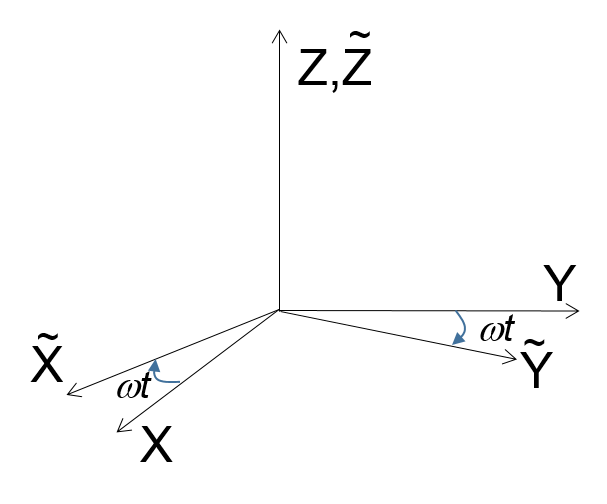
\includegraphics[scale=0.7]{rotating_frame.png}
%\end{figure}
%%%%% END OF FIGURE
%
% Magnetization in the rotating frame precesses with its respective Larmor frequency around the direction of an effective magnetic field $\bm{H_{eff}}$ given by Eq.\ref{eq:H_eff}. For a field oscillating on resonance (i.e. exactly at the Larmor frequency) the effective field has components only along $x,y$-axis. If the oscillating magnetic field is applied for a brief period of time $t_p$, i.e. in a form of a pulse, the effect of such a pulse is a rotation of magnetization by a finite angle:
%
%\begin{equation}
%\theta = \gamma H_1 t_p
%\end{equation}
%
%Now if a starting magnetization of our sample is directed along $z$-axis, a pulse having a nominal flip angle $\pi/2$ with an effective field $\bm{H_{eff}}$ along the $x$-axis in the rotating frame, would align the magnetization vector along the $y$-axis. When the oscillating field is switched off, the magnetization would stay stationary in the rotating frame which means it will precess with its own Larmor frequency in the laboratory frame.
%
%%%%% FIGURE SAMPLE COIL
%\begin{figure}[ht]
%\caption{(A) A sample with magnetization $\bm{M}$ placed inside a coil. (B) FID following a $\pi/2$ pulse is being Fourier transformed to give a NMR spectrum.}
%\label{fig:sample_coil}
%\centering
%%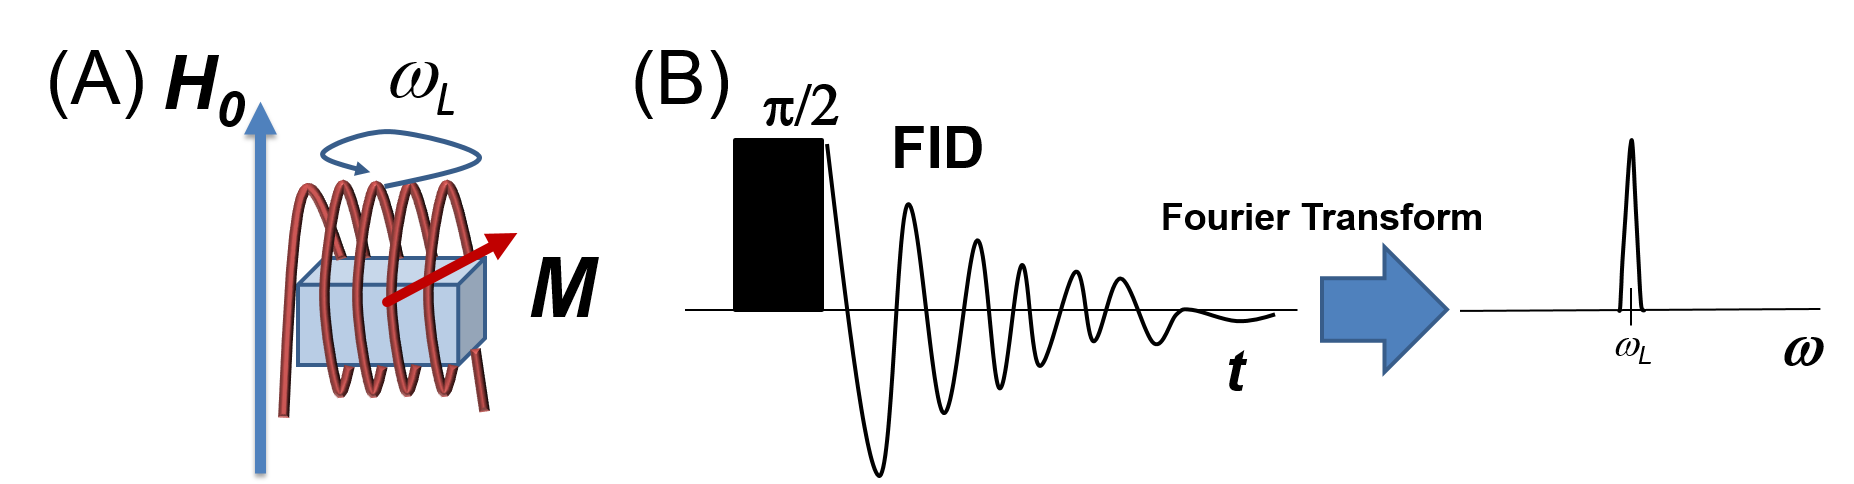
\includegraphics[scale=0.5]{sample_coil.png}
%\end{figure}
%%%%% END OF FIGURE
%
%The oscillating magnetic field in NMR spectrometers is usually produced by a coil would around as shown in Fig.\ref{fig:sample_coil}A. Moreover the same coil is being used for the detection of NMR signals. The precessing magnetization produces magnetic field, oscillating with the Larmor frequency and therefore produces oscillating  magnetic field flux through the coil. The oscillating magnetic field flux in turn induces small voltages across the coil which can be detected. The detection of NMR signals in almost all modern day spectrometers (and MRI machines) is based on this simple scheme. The signal following a $\pi/2$ pulse is called free induction decay or FID(it does not last forever as will be shown later ), which Fourier transform gives a NMR spectrum as shown in Fig.\ref{fig:sample_coil}B.
%
%Detection of FID following a single pulse often provides very limited information. The power of modern magnetic resonance lies in the design of specialized trains of pulses or pulse sequences, which can reveal a variety of interactions and connections of the materials under study (an example of 2D spectrum produced by a pulse sequence is shown in Fig.\ref{fig:fibrils}B).
%
%\textbf{Further reading:} Slichter, Ch. 2.1, 2.4 
%
%\section{Comment on NMR equipment.}
%
%It goes without saying that design of equipment for NMR and MRI is a field dominated by physicists and electrical engineers. Building novel instruments is a continuing process and there are a number of scientific groups as well as companies in industry working on the development of novel magnetic resonance instruments.
%  Development of coils and detection electronics, magnets and various accessories is currently carried out in several large and small companies around the world. Quite an extensive list is compiled at this webpage: \url{http://www.ebyte.it/library/NmrMriCompanies.html}. A number of particular examples of products will be given in some later sections.
% Furthermore, it should always be kept in mind that all the development is strongly supported by a progress in software controlling the NMR/MRI signal acquisition, processing, analysis. All of that could be an excellent area where physicists may apply their skills and knowledge.
%
%\section{Relaxation.}
% The spin system is never completely isolated from its environment, implying an energy exchange between the spins and molecular motions. The effect of coupling between spins and molecular motions can be explained as follows.
% All magnetic species around a spin create a local magnetic field $B_{loc}$ for instance due to interaction of magnetic dipolar moments. In turn, motions produce fluctuations of $B_{loc}(t)$. A careful look at the Eqs.\ref{eq:oscillating_field} and \ref{eq:probability} reveals that fields fluctuating at a resonant frequency cause transitions in a spin system, which essentially is an energy exchange between the spin system and the environment. These processes drive the spin system towards thermal equilibrium with the environment. For instance a spin-$\frac{1}{2}$ system at thermal equilibrium would have Bolzmann distribution of populations at levels $m_z=\frac{1}{2}$ and $m_z=-\frac{1}{2}$:
%
%\begin{equation}
%\begin{array} {lcl} \label{eq:populations}
%p_{\frac{1}{2}} &=& \dfrac{\exp{ (-\frac{\gamma \hbar H_0}{2kT}) }}{\exp{ (\frac{\gamma \hbar H_0}{2kT}) }+\exp{ (-\frac{\gamma \hbar H_0}{2kT} )}} \\
%p_{-\frac{1}{2}} &=& \dfrac{\exp{ (\frac{\gamma \hbar H_0}{2kT}) }}{\exp{ (\frac{\gamma \hbar H_0}{2kT}) }+\exp{ (-\frac{\gamma \hbar H_0}{2kT} )}}
%\end{array}
%\end{equation}
% At thermal equilibrium magnetization retains only its $z$-component $M_{z,eq} = \gamma \hbar N (p_{\frac{1}{2}} - p_{\frac{1}{2}}) $, where $N$ - total number of spins. In the classical model of precessing magnetization, Eq.\ref{precession} can be modified to include the interaction with lattice in a form of so called Bloch equations:
%\begin{equation}
%\begin{array}{lcl}
%\dfrac{dM_x}{dt} & = & \omega_0 M_y - \dfrac{M_x}{T_2}  \\
%\dfrac{dM_y}{dt} & = & -\omega_0 M_x - \dfrac{M_y}{T_2} \\
%\dfrac{dM_z}{dt} & = & \dfrac{M_{z,eq}-M_z}{T_1} 
%\end{array}
%\end{equation} 
%
%Here parameters $T_1$ and $T_2$ are called longitudinal and transversal relaxation times respectively and they show the rates at which magnetization approaches equilibrium. As mentioned above $T_1$ and $T_2$ both depend on the motions of a nucleus carrying the spin (i.e. a molecule with this spin) and the motions of environment. The values of $T_1$ and $T_2$ therefore report on the type of those motions and can explain the properties of material. 
%$T_1$ measurements can be carried out by following the recovery of magnetization after a $\pi$ pulse as schematically shown in Fig.\ref{fig:mz_buildup}. 
%
%%%%% FIGURE MZ_BUILDUP
%\begin{figure}[ht]
%\caption{Buildup of $M_z$ magnetization as a function of time after applying of a $\pi$ pulse at a time moment A, the following exponential recovery of magnetization is shown at moments B,C,D.}
%\label{fig:mz_buildup}
%\centering
%%\includegraphics[scale=0.3]{mz_buildup.png}
%\end{figure}
%%%%% END OF FIGURE 
%
%\textbf{Further reading:} Slichter, Ch. 1.3, 2.7
%
%
%\section{Comment of $T_1$ and $T_2$ measurements and their use in physical sciences.}
%  Relaxation times  $T_1$ and $T_2$ are probably the most commonly measured properties which are being used in a variety of industrial applications. 
%  
%  Quality control is very important in many of industries. Simple spectral and relaxation information provides important clues about the progress of a chemical procedure. For example Bruker company offers a variety of specialized NMR spectrometers designed for a particular task: analysis of polymers, food products, toothpaste and so on.
%  
%  Oil companies are  interested in getting accurate information on the soil porosity and fluid composition and content in their oil reservoirs. A special technique called NMR-logging essentially measures relaxation times which report on the sought properties using a probe lowered into a drilled well to various depths.
%  
% A new startup company T2Biosystems has recently introduced an instrument which uses relaxation effects of magnetic nanoparticles coated with some target-specific coatings. When a target is present, the particles bind and cluster around it, which in turn changes the relaxation properties of water molecules in the sample. The system is being used to detect pathogens such as bacteria and fungi in blood samples and could actually help in telling doctors to administer antibiotics before a disease has developed into its full strength.
%\section{Imaging.}
%
% As shown above, the Larmor frequency is proportional to the magnitude of the magnetic field. If one applies a constant gradient along some axis the Larmor frequency of nuclei becomes different at different physical locations within a sample:
% 
%\begin{equation}
%\omega(x,y,z) = \gamma (H_0 + G_x x + G_y y + G_z z),
%\end{equation}
%where $G_x$,$G_y$,$G_z$ is the magnetic field gradient, and $x$,$y$,$z$ are the coordinates within a sample.
%
%The NMR spectrum of a sample taken in the magnetic field gradient gives a projection of nuclei density onto the axis of NMR gradient. Fig.\ref{fig:MRI}A shows schematically four projections of the same object taken along different gradient axis. The full 3D image can be reconstructed from a large enough number of such projections along various axis. This forms the basis of magnetic resonance imaging. 
%
%%%%% FIGURE MRI
%\begin{figure}[ht]
%\caption{(A) Projections along various magnetic field gradients \textit{(Source: P.C. Lauterbur Nature 1973, 242, p.191)}. (B) Whole body MRI scan. \textit{(Source: S. Eustace, E.Nelson BMJ 2004, 328, p.1387) }. (C) Head MRI scan \textit{(Source: MRI brain scans database \url{http://adni.loni.usc.edu/data-samples/mri/} )} }
%\label{fig:MRI}
%\centering
%%\includegraphics[scale=0.45]{MRI.png}
%\end{figure}
%%%%% END OF FIGURE 
%
%  The projection reconstruction approach has been used in the early days of magnetic resonance imaging and still is being applied in electron paramagnetic resonance imaging (i.e. using magnetic resonance on unpaired electrons). However, modern systems use elaborated pulse sequences to acquire NMR signals necessary for image reconstruction.
%  In addition, constructing an image based solely on the number of magnetic moments in a volume is often not a very productive approach, because actual differences in the number of nuclei is often not very large (especially in medical applications), instead using differences in $T_1$ and $T_2$ relaxation times could produce images with better contrast.
%  
%\textbf{Further reading:} Slichter, Ch. 7.28, 2.7
%  
%  
%\section{Comment on MRI applications.}
%  1. Human body consists of water and significant amount of organic tissue, both of which are very rich in protons \textsuperscript{1}H. This is why \textsuperscript{1}H-based MRI enables medical applications, which have already become a routine diagnostic method, and Fig.\ref{fig:MRI}B,C shows examples of typical scans for a whole body and a head respectively. Lots of large and small companies work in this market offering various products such as hardware for signal acquisition, design of novel acquisition schemes, design of software for controlling the experimental setup and image reconstruction.
%  
%  Besides large established players (Siemens, Phillips, GE etc.) there are also some smaller companies, which often offer very specialized services, for instance, a small UK-based startup called "ImageAnalysis" have created software which uses some complex algorithms of image analysis to aid clinicians in tracking the changes and evaluating the effects of treatment.
%  There is a number of medium and small size companies which produce MRI scanners for preclinical (i.e. non-human) MRI, work on low-cost MRI and MRI of body parts. 
%
%  2. One of the most recent advances in MRI is a so called functional MRI (fMRI), which already made a very large impact in imaging brain activity. It turns out that active parts of the brain experience enhanced blood flow, carrying more oxygen. Oxygen, in turn, affects the relaxation times of water molecules around it. Therefore parts of the brain, active upon some stimulus "light up" in the MRI image, giving ideas to neuroscientists about what is going on in human brain.
%
%  3. However, researchers should not get locked into an idea that MRI is solely for medical applications. In fact, it is used quite a lot in material science, where one need to understand what happens inside non-transparent objects, such as chemical reactors or batteries.
%  
%\section{Hyperpolarization.}
%
%  One of the most significant problems in magnetic resonance is its relatively poor sensitivity. On the general level, the very low sensitivity stems from  a very low energy quantum emitted by a spin, as well as a very low magnetization of a sample under typical conditions. For a spin-$\frac{1}{2}$ the magnetization would be given by a difference of a number of spin looking along the magnetic field $N_{\frac{1}{2}}$ and those looking in the opposite direction $N_{\frac{1}{2}}$, in other words:
%  \begin{equation}
%  M = \dfrac{\gamma \hbar}{2} ( N_{\frac{1}{2}} - N_{-\frac{1}{2}}) = \dfrac{\gamma \hbar N}{2}  (p_{\frac{1}{2}} - p_{-\frac{1}{2}}),  
%  \end{equation}
%  where $N$ is the total number of spins and $p_{\frac{1}{2}}$,$p_{-\frac{1}{2}}$ are levels populations as defined in Eq.\ref{eq:populations}. In fact, plugging in the numbers for typical magnetic fields used in NMR for protons one gets a relative level population difference which is called "polarization" on the order of $10^{-5}$, meaning that spins are not very well aligned with the magnetic field. Getting a totally 100\% polarized sample, where all the spins are facing one direction is the main goal of the field, because it would have dramatic consequences both for NMR and MRI.
%  
%  Quite a number of approaches are capable of producing the very high polarization. We will focus only one of them called dynamic nuclear polarization (DNP), which is based on transferring polarization from unpaired electrons onto coupled nuclei. One of the simplest DNP mechanisms is a so called "solid-effect". We will consider a system of one unpaired electron coupled to a nucleus. The Hamiltonian of such a system has the following form:
%  \begin{equation}
%  \hat H = \gamma_N \hbar H_0 I_z - \gamma_e \hbar H_0 S_z + \sum_{i,j}A_{i,j}I_i S_j,
%  \end{equation}
%where $\gamma_N$ and $\gamma_e$ are the gyromagnetic ratios for the nucleus and electron respectively, $\bm{I}$ and $\bm{S}$ - are the spin angular momentum operators for nucleus and electron, and $A_{i,j}$ is the tensor of coupling between the two spins (it is composed of magnetic interaction between magnetic dipoles of electron and nucleus and hyperfine interaction). For $S=I=\frac{1}{2}$ system this Hamiltonian gives rise to a 4-level system with eigenfunctions \textit{almost} corresponding to spin up and down states of electron and nucleus as shown schematically in Fig.\ref{fig:solid_effect}A. Since the gyromagnetic ratio of electron is ~660 times larger than that of a proton (which has the highest among all nuclei) at low temperatures the population of upper electron sublevels is close to zero, and only the lowest sublevels get populated.
%
%%%%% FIGURE SOLID EFFECT
%\begin{figure}[ht]
%\caption{(A) Level diagram for the solid-effect DNP and steps during polarization process. The red circles on the levels schematically denote relative populations at low temperatures. (B) stable radicals and biradicals commonly serving as sources of unpaired electrons. (C) Spectra of a proline molecule in a frozen water/glycerol solution with DNP-producing microwave irradiation and without it, temperature 90K, magnetic field 5T. Unpaired electrons were added in the form of nitroxide biradicals. Overall signal enhancement observed was $\epsilon \sim 240$.}
%\label{fig:solid_effect}
%\centering
%%\includegraphics[scale = 0.25]{solid_effect.png}
%\end{figure}
%%%%% END OF FIGURE
%  
%  In fact, the eigenstates are not actually pure $\vert \alpha \beta \rangle$  states, but always contain a little admixture of other functions. This makes flip-flop transitions (i.e. making a flip of an electron and a nucleus at once) allowed. By applying  irradiation to one of the flip-flop transitions, it is then possible to create very large non-equilibrium population difference on nuclear sublevels, as shown in diagram \ref{fig:solid_effect}A. One can see that while at the beginning the population of nuclear $\vert \alpha_N \rangle$ and $\vert \beta_N \rangle$ sublevels was almost the same, after irradiation an excess of $\vert \beta_N \rangle$ is created. The $T_{1,e}$ electron relaxation process finally equilibrates electron spins, whereas nuclei $T_1$ times are very long at low temperatures and have little effect. Unpaired electrons are quite common in many materials, however, most materials do not contain them, so usually they are added in the form of stable radicals similar to those shown in Fig.\ref{fig:solid_effect}B.
% 
%  Fig.\ref{fig:solid_effect}C shows the effect of DNP in frozen water/glycerol solution (though using some other mechanism) on the amplitude of NMR signals in a  sample of proline aminoacid. Here using of DNP allowed reducing the time necessary to signal acquisition by many orders magnitude. This huge factor comes about because while the signals grow by a factor of $\epsilon \sim 240$, the signal-to-noise grows depends on the number of NMR scans as $\sqrt{N_{scans}}$, which is why the time taking accumulation of the same signal-to-noise spectra with and without DNP decreases by a factor of $\sim 240^{2} \approx 57600$!
%  
%  Getting higher NMR signals in MRI is also a very desirable goal. A typical medical MRI scan takes about 30 minutes, so getting a scan in a shorter time could potentially be a game changer. It is pretty hard to do though, but recently people have made progress along this avenue.
%  
%  A rather interesting approach is to polarize the carbonyl \textsuperscript{13}C nucleus of a pyruvic acid. It turns out that metabolism of pyruvate varies in normal tissue and cancer tumor tissue. The polarized pyruvate is injected into an animal (or human) and its conversion into lactate can be tracked using MRI. While this approach is already being used for research purposes, it has a very good chance of finding its way into clinical practice.
%  
%  Hyperpolarization using DNP (and other approaches) is at the frontier of the magnetic resonance science, and University of Nottingham is very active in this area. There is a number of home-built DNP (and other hyperpolarization scheme) systems in the University of Nottingham (see university web pages about the work of Profs. Meersman, Owers-Bradly, K{\"o}ckenberger). Furthermore just recently an installation of two commercial DNP systems has been completed, one of the instruments dedicated to applications in NMR, the other one - to MRI applications.
%
%\section{Afterword.}
% Modern magnetic resonance is a very dynamic field, where lots of novel developments are coming up both in academic labs and industry. There is a huge number of ways, where physicists could apply their skills obtained during university training: they could work on the development of novel hardware and signal acquisition schemes, design the software for processing and analysis of NMR and MRI data, work on deeper understanding of a magnetic resonance theory, or study biophysical processes at the levels of an individual molecule or a whole human body.

\end{document}
